% ---------------------------------------------------------------------------
% Reporte - Práctica 2 - Estructuras de Datos y Algoritmos (EAFIT)
% Compila con:  pdflatex reporte.tex  (dos veces)  o  tectonic reporte.tex
% El documento inserta los .cpp con \lstinputlisting: los rangos de línea
% apuntan a los archivos reales de ../src (ver Anexo B).
% ---------------------------------------------------------------------------
\documentclass[11pt,a4paper]{article}

\usepackage{iftex}
\ifPDFTeX
  \usepackage[utf8]{inputenc}
  \usepackage[T1]{fontenc}
\fi
\usepackage[spanish,es-nodecimaldot]{babel}
\usepackage{lmodern}
\usepackage[margin=2.4cm]{geometry}
\usepackage{amsmath,amssymb}
\usepackage{graphicx}
\usepackage{booktabs}
\usepackage{array}
\usepackage{xcolor}
\usepackage{listings}
\usepackage{enumitem}
\usepackage{caption}
\usepackage{fancyhdr}
\usepackage{titlesec}
\usepackage[hidelinks]{hyperref}

% ---------------------------- estilo del codigo ----------------------------
\definecolor{codebg}{RGB}{248,248,248}
\definecolor{codekw}{RGB}{0,80,150}
\definecolor{codecm}{RGB}{0,120,0}
\definecolor{codestr}{RGB}{170,40,40}
\definecolor{termbg}{RGB}{240,240,240}

\lstdefinestyle{cpp}{
  language=C++,
  basicstyle=\ttfamily\footnotesize,
  keywordstyle=\color{codekw}\bfseries,
  commentstyle=\color{codecm}\itshape,
  stringstyle=\color{codestr},
  numbers=left,
  numberstyle=\tiny\color{gray},
  numbersep=9pt,
  backgroundcolor=\color{codebg},
  frame=single,
  rulecolor=\color{gray!45},
  breaklines=true,
  breakatwhitespace=true,
  tabsize=4,
  showstringspaces=false,
  captionpos=b,
  xleftmargin=16pt,
  framexleftmargin=16pt,
  literate={á}{{\'a}}1 {é}{{\'e}}1 {í}{{\'i}}1 {ó}{{\'o}}1 {ú}{{\'u}}1 {ñ}{{\~n}}1 {Á}{{\'A}}1 {É}{{\'E}}1 {Í}{{\'I}}1 {Ó}{{\'O}}1 {Ú}{{\'U}}1 {Ñ}{{\~N}}1 {ü}{{\"u}}1 {Ü}{{\"U}}1
}

\lstdefinestyle{term}{
  basicstyle=\ttfamily\footnotesize,
  backgroundcolor=\color{termbg},
  frame=single,
  rulecolor=\color{gray!45},
  breaklines=true,
  columns=fullflexible,
  keepspaces=true,
  showstringspaces=false,
  xleftmargin=10pt,
  framexleftmargin=10pt,
  literate={á}{{\'a}}1 {é}{{\'e}}1 {í}{{\'i}}1 {ó}{{\'o}}1 {ú}{{\'u}}1 {ñ}{{\~n}}1 {Á}{{\'A}}1 {É}{{\'E}}1 {Í}{{\'I}}1 {Ó}{{\'O}}1 {Ú}{{\'U}}1 {Ñ}{{\~N}}1 {ü}{{\"u}}1 {Ü}{{\"U}}1
}

\captionsetup[lstlisting]{font=small,labelfont=bf}
\renewcommand{\lstlistingname}{Listado}
\addto\captionsspanish{\renewcommand{\tablename}{Tabla}}
\renewcommand{\lstlistlistingname}{Listado de códigos}

\titleformat{\section}{\normalfont\large\bfseries}{\thesection}{0.8em}{}
\titleformat{\subsection}{\normalfont\normalsize\bfseries}{\thesubsection}{0.8em}{}
\setlist[itemize]{topsep=2pt,itemsep=1pt,parsep=0pt,leftmargin=1.4em}
\setlist[enumerate]{topsep=2pt,itemsep=1pt,parsep=0pt,leftmargin=1.6em}

\pagestyle{fancy}
\fancyhf{}
\rhead{\small Práctica 2 --- EDA}
\lhead{\small Giraldo · Rojas · Cubaque}
\cfoot{\thepage}
\renewcommand{\headrulewidth}{0.3pt}

\newcommand{\arch}[1]{\texttt{#1}}


% ===========================================================================
\begin{document}

% babel-espanol convierte < y > en comillas latinas; aquí los necesitamos
% literales para escribir \texttt{<queue>} y los operadores del código.
\shorthandoff{<>}

% ------------------------------- portada -----------------------------------
\begin{titlepage}
\centering
{\scshape\large Universidad EAFIT\par}
\vspace{0.3cm}
{\large Estructuras de Datos y Algoritmos\par}
\vspace{2.2cm}
{\Huge\bfseries Práctica 2\par}
\vspace{0.6cm}
{\Large Navegador de rutas del Metro de Medellín\par}
\vspace{0.8cm}
{\large Grafos, Dijkstra, A*, rutas alternativas, puntos de\\ articulación y autocompletado en C++17\par}
\vfill
\begin{tabular}{r@{\hspace{0.6cm}}l}
\textbf{Profesor} & Germán A. Montoya O. \\
 & \texttt{gamontoyao@eafit.edu.co} \\[0.4cm]
\textbf{Estudiantes} & Juan David Giraldo \\
 & Daniel Rojas \\
 & Jeronimo Cubaque \\
\end{tabular}
\vfill
{\large Medellín, 2026\par}
\end{titlepage}

% ------------------------------- contenido ---------------------------------
\section{Qué hicimos}

La práctica pide un programa en C++ que cargue el grafo de un sistema de
transporte público, encuentre el camino de menor tiempo entre dos estaciones,
visualice la ruta y exporte el grafo con esa ruta seleccionada. Elegimos el Metro
de Medellín con las líneas A y B, los metrocables K, J, L, H y M y el tranvía de
Ayacucho (T-A): 46 estaciones y 8 líneas.

El programa se llama \arch{navegador} y se maneja con un menú de consola. Tiene
las cuatro funcionalidades mínimas y cinco adicionales:

\begin{itemize}
  \item carga del grafo desde dos archivos CSV;
  \item ruta de menor tiempo con Dijkstra y una \arch{priority\_queue};
  \item visualización de la ruta en un SVG escrito a mano e impresión de la ruta
        en consola;
  \item exportación del grafo y de la ruta a DOT y JSON;
  \item A* con heurística haversine y comparación contra Dijkstra;
  \item costo de transbordo modelando los nodos como pares (estación, línea);
  \item $k$ rutas alternativas con el algoritmo de Yen;
  \item simulación de estación cerrada y detección de puntos de articulación con
        DFS y \emph{low-link};
  \item autocompletado de estaciones con un Trie, sin distinguir tildes ni
        mayúsculas;
  \item una interfaz web (servidor HTTP con sockets y una página con el mapa
        interactivo) sobre el mismo motor.
\end{itemize}

\textbf{No se usó ninguna librería externa.} Todo el programa es C++17 con la
biblioteca estándar (contenedores, \arch{<queue>}, \arch{<set>}, \arch{<fstream>},
\arch{<random>} para el experimento de A* y \arch{<filesystem>} para crear la
carpeta de salida). El SVG, el DOT y el JSON se escriben carácter por carácter
desde el programa; no hay dependencias de graficación.

\begin{center}
\arch{src/graph.hpp} · \arch{src/graph.cpp} · \arch{src/algorithms.hpp} ·
\arch{src/algorithms.cpp} · \arch{src/trie.hpp} · \arch{src/io.hpp} ·
\arch{src/io.cpp} · \arch{src/main.cpp} · \arch{tests/test\_main.cpp}
\end{center}

La red que modelamos es un árbol: 46 estaciones conectadas con 45 tramos, sin
ciclos. Eso tiene consecuencias que aparecen varias veces en el informe (entre
dos estaciones existe un único camino simple) y las discutimos en la
sección~\ref{sec:limitaciones}.

% ===========================================================================
\section{Instalación y ejecución}
\label{sec:ejecucion}

No hay librerías externas que instalar: todo se resuelve con la biblioteca
estándar. Se necesita un compilador de C++17 y CMake. El proyecto compila igual
en Windows y en Linux. En Windows hace falta Visual Studio con la carga de
trabajo \emph{Desarrollo para el escritorio con C++}, o MinGW-w64; en Linux,
\arch{g++} y \arch{cmake} (aquí se midió con g++ 14.2.0 y CMake 3.31.6).

El servidor web usa sockets POSIX en Linux y Winsock en Windows, con un bloque
\arch{\#ifdef \_WIN32} en \arch{src/servidor.cpp} y el enlace a \arch{ws2\_32} en
el \arch{CMakeLists.txt}. El mismo código y los mismos comandos sirven en los dos
sistemas; solo cambia la ruta del ejecutable.

\subsection*{Compilar}
Desde la carpeta del proyecto, en Windows con ``Símbolo del sistema'' o
PowerShell y MinGW-w64 (hay que tener \arch{g++} y \arch{mingw32-make} en el
\arch{PATH}):

\begin{lstlisting}[style=term]
cmake -S . -B build -G "MinGW Makefiles"
cmake --build build
\end{lstlisting}

Si \arch{cmake} avisa de que no encuentra el programa de compilación, MinGW no
está en el \arch{PATH}: Windows no trae compilador de C++ por defecto, así que
hay que instalarlo (winlibs o MSYS2) y añadir su carpeta \arch{bin} al
\arch{PATH} antes de repetir los comandos. El \arch{CMakeLists.txt} enlaza el
ejecutable de MinGW de forma estática, así que después no depende de las DLL de
la biblioteca estándar y se puede abrir desde cualquier carpeta.

El ejecutable queda en \arch{build\textbackslash{}navegador.exe}. Con Visual
Studio (carga de trabajo \emph{Desarrollo para el escritorio con C++}) se omite
el generador y se compila Release:

\begin{lstlisting}[style=term]
cmake -S . -B build
cmake --build build --config Release
\end{lstlisting}

y el ejecutable queda en la subcarpeta \arch{Release} de \arch{build}. El
\arch{CMakeLists.txt} fija el estándar C++17 y desactiva las extensiones del
compilador, y compila sin advertencias (Anexo~\ref{anexo:compila}). El proyecto
no incluye scripts de por medio: los dos comandos anteriores son todo lo
necesario.

\subsection*{Opción A: interfaz web}
Se levanta el servidor y se abre \arch{http://localhost:8080} en el navegador:

\begin{lstlisting}[style=term]
cd C:\ruta\a\practica2
build\navegador.exe --web
\end{lstlisting}

Hay que lanzarlo desde la carpeta del proyecto, porque el servidor busca
\arch{web\textbackslash{}index.html} relativo a la carpeta actual (y si no lo encuentra,
\arch{..\textbackslash{}web\textbackslash{}index.html}). Para usar otro puerto:
\arch{navegador.exe --web 9000}. El servidor escucha solo en
\arch{127.0.0.1}: la interfaz es local, así que no expone el puerto a la red ni
dispara el aviso del Firewall de Windows.

\subsection*{Opción B: solo consola (\arch{main})}
Sin \arch{--web}, el programa corre el menú interactivo de consola, que es el
\arch{main} de la práctica:

\begin{lstlisting}[style=term]
cd C:\ruta\a\practica2
build\navegador.exe
\end{lstlisting}

El menú tiene las siete
opciones: autocompletar con Trie, ruta más rápida con Dijkstra, A* contra
Dijkstra, rutas alternativas de Yen, simulación de estación cerrada, puntos de
articulación y exportación a DOT, JSON y SVG. La opción 7 crea
\arch{out}\textbackslash{} y escribe ahí \arch{route.dot}, \arch{route.json} y
\arch{route.svg}.

\subsection*{Pruebas y equivalencia en Linux}
Las pruebas con \arch{assert} se compilan y corren igual:

\begin{lstlisting}[style=term]
build\pruebas.exe         :: Windows (MinGW)
build\Release\pruebas.exe :: Windows (Visual Studio)
./build/pruebas           # Linux
\end{lstlisting}

En Linux los mismos pasos son:

\begin{lstlisting}[style=term]
cmake -S . -B build && cmake --build build -j4
./build/navegador                # menú de consola
./build/navegador --web          # interfaz web en http://localhost:8080
./build/pruebas                  # pruebas
\end{lstlisting}

% ===========================================================================
\section{Los datos}
\label{sec:datos}

\subsection{Los dos CSV}

\arch{data/stations.csv} tiene una fila por estación con cinco columnas:
\arch{id}, \arch{nombre}, \arch{linea}, \arch{lat} y \arch{lon}. El \arch{id} es
un identificador corto y sin espacios (\arch{san\_antonio}, \arch{la\_estrella})
que se usa en el otro archivo. Cuando una estación pertenece a varias líneas, la
columna \arch{linea} las trae separadas por una barra vertical: San Antonio es
\arch{A|B|T-A}, Acevedo es \arch{A|K}.

\arch{data/edges.csv} tiene una fila por tramo con \arch{origen},
\arch{destino} y \arch{minutos}. Los extremos son ids de estación y el tramo se
considera en los dos sentidos. La línea del tramo no se guarda porque se deduce:
las dos estaciones comparten exactamente una línea, y esa es la del tramo. Así el
archivo se mantiene en las tres columnas que pide la práctica.

Los nombres y las coordenadas salen de los artículos de Wikipedia del
\emph{Metro de Medellín}, del \emph{Metrocable de Medellín} y de la lista de
estaciones; las coordenadas están en grados decimales con cinco cifras (unos
pocos metros de precisión). No son lecturas de un levantamiento topográfico: son
las coordenadas publicadas de cada estación y sirven para dibujar y para estimar
distancias, no para navegación real.

\subsection{Los tiempos son estimados}

Los tiempos entre estaciones \textbf{no son datos oficiales del Metro}. Como el
sistema no publica la matriz de tiempos entre todas las estaciones, los
calculamos con la distancia geográfica y una velocidad comercial por tipo de
línea:
\begin{equation}
  t_{uv} = \frac{60 \cdot d_{uv}}{v_{\ell}} \quad \text{minutos},
  \label{eq:tiempo}
\end{equation}
donde $d_{uv}$ es la distancia haversine entre las estaciones $u$ y $v$ en
kilómetros y $v_{\ell}$ es la velocidad comercial de la línea $\ell$ en km/h. La
velocidad incluye las paradas y el tiempo de subida y bajada, por eso es bastante
menor que la velocidad máxima del tren (80 km/h en las líneas A y B). Los valores
que usamos están en la tabla~\ref{tab:lineas}.

\begin{table}[htbp]
\centering
\small
\begin{tabular}{llrrrr}
\toprule
Línea & Tipo & Estaciones & Longitud (km) & Tiempo (min) & $v_\ell$ (km/h) \\
\midrule
A     & Metro      & 21 & 24,17 & 40,2 & 36 \\
B     & Metro      &  7 &  5,19 & 10,1 & 31 \\
K     & Metrocable &  4 &  2,01 &  8,6 & 14 \\
J     & Metrocable &  4 &  2,69 & 11,5 & 14 \\
L     & Metrocable &  2 &  4,48 & 14,9 & 18 \\
H     & Metrocable &  3 &  1,43 &  5,3 & 16 \\
M     & Metrocable &  3 &  1,10 &  4,1 & 16 \\
T-A   & Tranvía    &  9 &  3,80 & 13,4 & 17 \\
\bottomrule
\end{tabular}
\caption{Las ocho líneas del grafo: estaciones, longitud geográfica sumando los tramos, tiempo total que sale de la ecuación~\eqref{eq:tiempo} y velocidad usada. Las 53 estaciones de la columna suman los pares (estación, línea); las estaciones distintas son 46 porque seis estaciones son intercambiadores.}
\label{tab:lineas}
\end{table}

Como control, la suma de los tramos de la línea A da 40,2 minutos y el Metro
publica 42 minutos para el recorrido completo Niquía--La Estrella; en la línea B
salen 10,1 contra los 10,5 minutos publicados. La ecuación reproduce los tiempos
de recorrido completo con un error del 5\,\% o menos, que es más que suficiente
para comparar rutas. Aun así, en todo el informe se insiste en lo mismo: son
\textbf{estimaciones}, no horarios.

\subsection{Distancia haversine}

La distancia entre dos coordenadas se calcula con la fórmula haversine, que trata
la Tierra como una esfera de radio $R = 6371$ km:
\begin{equation}
  d = 2R \arcsin\!\sqrt{\operatorname{sen}^2\!\left(\frac{\Delta\varphi}{2}\right)
      + \cos\varphi_1 \cos\varphi_2\,
        \operatorname{sen}^2\!\left(\frac{\Delta\lambda}{2}\right)},
\end{equation}
con $\varphi$ la latitud y $\lambda$ la longitud en radianes. La usamos en dos
lugares: para estimar los tiempos de la ecuación~\eqref{eq:tiempo} y como base de
la heurística de A* (sección~\ref{sec:astar}).

% ===========================================================================
\section{El grafo}

\subsection{El modelo: nodos (estación, línea)}

Si se modela cada estación como un nodo, un viaje que cambia de línea no cuesta
nada: llegar a San Antonio en la línea A y salir en la T-A queda como pasar por el
mismo nodo. Para poder cobrar el transbordo, el grafo que construimos es el
\emph{grafo expandido}: un nodo por cada par (estación, línea). San Antonio
aparece tres veces (San Antonio-A, San Antonio-B, San Antonio-T-A) y las tres
copias se conectan entre sí con aristas de transbordo que cuestan la penalización
configurada.

Con eso quedan $V = 53$ nodos y $E = 106$ aristas dirigidas: 45 tramos en cada
sentido ($2 \times 45$) y 16 aristas de transbordo (Acevedo, San Antonio, San
Javier, Santo Domingo Savio, Oriente y Miraflores, contando San Antonio tres
veces por tener tres líneas).

\begin{table}[htbp]
\centering
\small
\begin{tabular}{lrl}
\toprule
Estructura & Definición & Uso \\
\midrule
\arch{Estacion} & id, nombre, lat, lon, líneas & datos del CSV \\
\arch{Linea}    & código y color & colores del SVG \\
\arch{Nodo}     & par (estación, línea) & vértice del grafo \\
\arch{Arista}   & destino, minutos, esTransbordo & lista de adyacencia \\
\arch{Graph}    & los cuatro vectores anteriores & el grafo completo \\
\bottomrule
\end{tabular}
\caption{Las cuatro estructuras de \arch{graph.hpp} y la clase que las agrupa. Son \arch{struct} con datos públicos: no hay jerarquías ni métodos virtuales.}
\end{table}

\lstinputlisting[float=tbp,style=cpp,caption={\arch{src/graph.hpp}, líneas 8--35: las estructuras de datos del grafo.},label={lst:graph},firstline=8,lastline=35,firstnumber=8]{../src/graph.hpp}

\paragraph{Listas de adyacencia.}
El grafo se guarda como \arch{std::vector<std::vector<Arista>>}, un vector de
listas de adyacencia. Para un grafo con $V$ vértices y $E$ aristas ocupa
$O(V+E)$ de memoria y recorrer los vecinos de un nodo cuesta $O(\text{grado})$,
que es exactamente lo que necesitan Dijkstra y A*: en cada paso revisan las
aristas que salen del nodo que acaban de cerrar. Una matriz de adyacencia
costaría $O(V^2)$ y en cada paso habría que revisar $V$ posiciones, casi todas
vacías.

\subsection{La carga del CSV}

\lstinputlisting[float=tbp,style=cpp,caption={\arch{src/io.cpp}, líneas 119--171: creación de los nodos (estación, línea), de los tramos y de las aristas de transbordo.},label={lst:carga},firstline=119,lastline=171,firstnumber=119]{../src/io.cpp}

\paragraph{Los nodos (119--125).}
Por cada estación se crea un nodo por línea y se guardan en el mismo orden, de
modo que el nodo $k$ del vector \arch{nodos} se puede buscar después con
\arch{Graph::nodo(estacion, linea)}, que recorre el vector linealmente. Con 53
nodos esa búsqueda es gratis y no vale la pena una tabla hash.

\paragraph{Los tramos (127--159).}
Cada fila de \arch{edges.csv} se convierte en dos aristas, una por sentido, sobre
la línea que comparten las dos estaciones (\arch{std::find} sobre el vector de
líneas de la estación destino). Si una fila menciona una estación que no existe,
se cuenta y se avisa por \arch{cerr} al final, en vez de meter un nodo inválido.

\paragraph{Los transbordos (161--171).}
Por cada estación con más de una línea se agregan todas las aristas ordenadas
entre sus copias, cada una con la penalización \arch{transbordo} que llega como
parámetro de \arch{cargarGrafo}. Con penalización 0 las aristas existen y cuestan
cero; así el modelo se puede apagar desde el menú sin tocar el código. Al final se
calcula una vez la velocidad máxima del grafo, que A* reutiliza en todas las
búsquedas.

% ===========================================================================
\section{Dijkstra}

\paragraph{La idea.}
Se mantiene para cada nodo el mejor tiempo conocido desde el origen,
\arch{dist[v]}, que empieza en infinito salvo el origen (0). En una cola de
prioridad se guardan los candidatos (costo, nodo) y siempre se saca el más
barato. Como todos los costos son positivos, cuando un nodo sale del heap su
\arch{dist} ya es el definitivo: no hay forma de llegar más barato por un camino
que pase por nodos más caros. Ese es el argumento de correctitud y depende de que
no haya aristas negativas; nuestros minutos siempre son $\geq 0$.

\lstinputlisting[float=tbp,style=cpp,caption={\arch{src/algorithms.cpp}, líneas 53--109: Dijkstra con \arch{priority\_queue}. La versión de la línea 111 es un envoltorio para un origen y un destino.},label={lst:dijkstra},firstline=53,lastline=109,firstnumber=53]{../src/algorithms.cpp}

\paragraph{El heap (68).}
\arch{std::priority\_queue} con \arch{std::greater} es un montículo binario
mínimo: insertar y sacar el mínimo cuestan $O(\log V)$. Esa es la estructura que
pide el algoritmo; con una cola normal habría que buscar el mínimo recorriendo la
cola en cada paso y el costo subiría a $O(V^2)$.

\paragraph{Borrado perezoso (85).}
El heap no permite disminuir la clave de una entrada, así que cuando un nodo
mejora se inserta una entrada nueva y la vieja se descarta al sacarla
(\arch{if (actual.first > dist[u]) continue}). Cada arista puede meter a lo sumo
una entrada, de modo que el heap nunca pasa de $E$ elementos.

\paragraph{Varios orígenes y varios destinos (70--78).}
Un estación puede tener varias copias (una por línea), así que en vez de correr
Dijkstra una vez por combinación, el heap arranca con todas las copias del origen
a costo 0 y la búsqueda termina cuando sale la primera copia del destino. Es la
misma cantidad de trabajo que un Dijkstra normal y evita repetir la búsqueda hasta
nueve veces por consulta.

\paragraph{Costo.}
Con listas de adyacencia y heap, $O((V+E)\log V)$; con $V=53$ y $E=106$ son
unos pocos miles de operaciones, o sea microsegundos. La memoria es $O(V)$ para
\arch{dist} y \arch{previo}.

\paragraph{Verificación a mano.}
Antes de confiar en el programa sumamos a mano las aristas del CSV. Cuatro rutas
quedaron fijas en \arch{tests/test\_main.cpp} como referencia:

\begin{center}
\small
\begin{tabular}{llrr}
\toprule
Ruta & Camino & Suma a mano (min) & Programa \\
\midrule
Niquía → La Estrella      & 20 tramos de la línea A & 40,2 & 40,2 \\
Niquía → San Antonio      & 10 tramos de la línea A & 18,6 & 18,6 \\
Universidad → Poblado     & 8 tramos de la línea A  & 11,1 & 11,1 \\
San Javier → Santo Domingo & B + A + K, 2 transbordos & 35,5 & 35,5 \\
\bottomrule
\end{tabular}
\captionof{table}{Rutas sumadas a mano sobre \arch{edges.csv} contra lo que devuelve el programa. La de San Javier incluye $3$ minutos por cada uno de los dos transbordos.}
\end{center}

% ===========================================================================
\section{A*}
\label{sec:astar}

\paragraph{La idea.}
A* es Dijkstra con una estimación del costo que falta. En vez de ordenar el heap
por el costo acumulado $g(v)$, lo ordena por $f(v) = g(v) + h(v)$, donde $h(v)$
es una cota inferior del tiempo que falta para llegar al destino. Si $h$ nunca
sobreestima, el primer destino que sale del heap sigue siendo el óptimo y se
expanden menos nodos, porque el heap prefiere los que van en dirección al destino.

\paragraph{La heurística.}
Usamos la distancia en línea recta dividida por la velocidad máxima de la red:
\begin{equation}
  h(v) = \frac{d_{\text{haversine}}(v, t)}{v_{\max}}, \qquad
  v_{\max} = 1{,}05 \cdot \max_{e \in E} \frac{d_e}{t_e}.
  \label{eq:heuristica}
\end{equation}
La velocidad máxima se mide sobre las mismas aristas del archivo, y el 5\,\% de
margen absorbe el redondeo a una décima de minuto con que se guardaron los
tiempos.

\paragraph{Por qué es admisible.}
Para cualquier camino $v = x_0, x_1, \dots, x_k = t$ el costo real es
$\sum_i t_{x_i x_{i+1}} = \sum_i d_i / v_i$. Como $v_i \leq v_{\max}$ para toda
arista, ese costo es mayor o igual que $\sum_i d_i / v_{\max}$, y por la desigualdad
triangular de la distancia geográfica $\sum_i d_i \geq d_{\text{haversine}}(v,t)$.
Entonces
\begin{equation}
  h(v) = \frac{d(v,t)}{v_{\max}} \;\leq\; \frac{\sum_i d_i}{v_{\max}}
       \;\leq\; \sum_i \frac{d_i}{v_i} = h^*(v),
\end{equation}
es decir, la heurística nunca se pasa del costo real. Además es consistente
($h(u) \leq t_{uv} + h(v)$) por la misma desigualdad triangular, así que cada nodo
se cierra una sola vez y no hace falta reabrirlo.

\lstinputlisting[float=tbp,style=cpp,caption={\arch{src/algorithms.cpp}, líneas 115--191: A*. La heurística se calcula una vez por nodo (131--142) y el resto es el mismo esqueleto de Dijkstra con $f = g + h$.},label={lst:astar},firstline=115,lastline=191,firstnumber=115]{../src/algorithms.cpp}

\paragraph{La heurística precalculada (136--148).}
Calcular $h$ cuesta dos senos y dos cosenos, mucho más que revisar un vecino. Por
eso se calcula una vez para los 53 nodos y se guarda en un vector; el bucle del
heap solo consulta \arch{heuristica[v]}. En un grafo de este tamaño ese
precálculo es la mitad del tiempo de la búsqueda, y lo decimos tal cual en los
resultados.

\paragraph{El conjunto cerrado (163--168).}
Con heurística consistente no hace falta volver a abrir un nodo ya cerrado, así
que se marca en un \arch{vector<char>} y las entradas repetidas del heap se
ignoran.

\subsection{A* contra Dijkstra}

La opción 3 del menú corre los dos algoritmos sobre el mismo par y después repite
el experimento con 20 pares aleatorios de estaciones (semilla fija 12345, para que
la tabla se pueda reproducir). Para el par Niquía--La Estrella, que es el camino
más largo de la red:

\begin{lstlisting}[style=term]
Dijkstra: costo 40.2 min, 50 nodos explorados
A*:       costo 40.2 min, 22 nodos explorados
Promedio de 200 corridas: Dijkstra 0.9 us, A* 2.7 us
\end{lstlisting}

\begin{table}[htbp]
\centering
\footnotesize
\begin{tabular}{rlrrrr}
\toprule
\# & Par & Costo D (min) & Costo A* (min) & Nodos D & Nodos A* \\
\midrule
 1 & Bicentenario → San José     &  2,9 &  2,9 &  4 &  3 \\
 2 & Poblado → Universidad       & 11,1 & 11,1 & 16 &  9 \\
 3 & Prado → Bello               & 14,5 & 14,5 & 29 &  8 \\
 4 & Parque Berrío → El Pinal    & 17,8 & 17,8 & 38 & 25 \\
 5 & San Javier → Floresta       &  3,5 &  3,5 &  4 &  4 \\
 6 & Andalucía → Buenos Aires    & 27,1 & 27,1 & 31 & 24 \\
 7 & Loyola → Cisneros           & 14,7 & 14,7 & 20 & 16 \\
 8 & Juan XXIII → Bicentenario   & 24,9 & 24,9 & 23 & 20 \\
 9 & Oriente → Envigado          & 31,1 & 31,1 & 40 & 26 \\
10 & Juan XXIII → Hospital       & 23,6 & 23,6 & 20 & 16 \\
11 & Oriente → Pabellón del Agua & 10,2 & 10,2 & 12 & 10 \\
12 & Loyola → Bello              & 29,8 & 29,8 & 41 & 28 \\
13 & Niquía → Industriales       & 22,0 & 22,0 & 20 & 14 \\
14 & Tricentenario → Itagüí      & 26,1 & 26,1 & 43 & 15 \\
15 & Industriales → Miraflores   & 15,1 & 15,1 & 28 & 17 \\
16 & Juan XXIII → Popular        & 39,5 & 39,5 & 47 & 32 \\
17 & Miraflores → Pabellón del Agua & 5,5 & 5,5 & 10 & 7 \\
18 & San José → Santa Lucía      & 12,6 & 12,6 & 27 & 14 \\
19 & Loyola → El Pinal           &  7,2 &  7,2 &  9 &  7 \\
20 & Arví → Madera               & 32,4 & 32,4 &  9 &  8 \\
\midrule
   & Promedio                    & 18,6 & 18,6 & 23 & 15 \\
\bottomrule
\end{tabular}
\caption{Los 20 pares aleatorios de la opción 3. El costo es idéntico en los 20 (diferencia máxima $0{,}000$ minutos) y A* explora en promedio el 64,3\,\% de los nodos de Dijkstra.}
\label{tab:astar}
\end{table}

\paragraph{Lo que muestran los números.}
El costo es el mismo en los 20 pares, que es la propiedad que tiene que cumplir
una heurística admisible, y A* explora en promedio 15 nodos contra 23 de
Dijkstra. El ahorro depende del par: entre estaciones vecinas es nulo (los dos
algoritmos exploran 4 nodos) y en los recorridos largos es grande (Tricentenario
→ Itagüí: 43 contra 15), porque la heurística descarta las ramas que se alejan del
destino.

\paragraph{El tiempo no mejora, y es honesto decirlo.}
A* explora menos nodos pero tarda entre tres y cuatro veces más por consulta
(0,9 µs contra 2,7 µs). La razón es el tamaño del grafo: calcular las 53
distancias para la heurística cuesta más que expandir las 8 o 10 aristas que
Dijkstra revisa de más. Con 53 nodos, el trabajo ahorrado es del orden de
decenas de operaciones y el de la heurística es del orden de cientos. La ganancia
en nodos explorados es la que importa en redes grandes, donde cada nodo tiene
muchos vecinos y el factor de ramificación castiga a Dijkstra; aquí el grafo es
diminuto y el efecto se ve en el conteo, no en el reloj.

% ===========================================================================
\section{Costo de transbordo}

\paragraph{El modelo.}
Como los nodos son pares (estación, línea), cambiar de línea es una arista con
costo $p$, la penalización configurable en minutos. La opción 8 del menú la cambia
(por defecto 3,0 min) y recarga el grafo con el nuevo valor. El modelo se puede
apagar con $p = 0$: las aristas siguen existiendo y cuestan cero.

\paragraph{Un ejemplo.}
San Javier está en la B y en la J; Santo Domingo Savio en la K y en la L. Para ir
de San Javier a Santo Domingo Savio el camino es B hasta San Antonio, A hasta
Acevedo y K hasta Santo Domingo, con dos transbordos de 3 minutos:

\begin{lstlisting}[style=term]
Ruta San Javier -> Santo Domingo Savio
  San Javier
  Santa Lucia  [Linea B]  2.2 min
  ...
  San Antonio  [Linea B]  10.1 min
  -- transbordo a Linea A (+3.0 min) en San Antonio
  ...
  Acevedo  [Linea A]  23.9 min
  -- transbordo a Linea K (+3.0 min) en Acevedo
  ...
  Santo Domingo Savio  [Linea K]  35.5 min
Total: 35.5 min | 16 tramos | 2 transbordos | 17 estaciones
\end{lstlisting}

Con la penalización en 0 el mismo recorrido cuesta 29,5 min: exactamente los
6 minutos de los dos transbordos. Ese es el efecto que se busca, y es la razón por
la que el transbordo se modela en el grafo y no como una suma al final: sumarlo
después de calcular la ruta sería cobrar por una decisión que el algoritmo ya
tomó sin tenerla en cuenta.

\paragraph{Costo.}
El grafo pasa de 53 nodos y 90 aristas de viaje a 106 aristas en total, un
aumento constante que no cambia ninguna complejidad: las búsquedas siguen siendo
$O((V+E)\log V)$ con $V = 53$ y $E = 106$.

% ===========================================================================
\section{Rutas alternativas (Yen)}

\paragraph{La idea.}
Yen calcula los $k$ caminos más cortos sin ciclos de forma iterativa: el primero
es el de Dijkstra; para el siguiente se toma la última ruta aceptada, se corta en
cada uno de sus nodos y se busca un desvío mínimo desde ese punto hasta el destino
prohibiendo las aristas que ya usaron las rutas aceptadas y los nodos de la raíz
(para no repetir estaciones). Todos los desvíos candidatos se guardan en un
\arch{std::set} ordenado por costo y en cada iteración se acepta el más barato que
no esté repetido.

\lstinputlisting[float=tbp,style=cpp,caption={\arch{src/algorithms.cpp}, líneas 197--274: Yen. Cada desvío es un Dijkstra con aristas y nodos bloqueados (\arch{Bloqueo}).},label={lst:yen},firstline=197,lastline=274,firstnumber=197]{../src/algorithms.cpp}

\paragraph{El bloqueo.}
\arch{Bloqueo} guarda dos cosas: un vector de nodos prohibidos y una matriz de
aristas prohibidas. El mismo tipo lo usan Dijkstra y A* para la simulación de
estación cerrada, así que un solo mecanismo resuelve las dos funcionalidades.

\paragraph{Costo.}
Cada desvío es un Dijkstra, y por cada ruta se prueban a lo sumo $n$ desvíos,
con $n$ el largo de la ruta: $O(k \cdot n \cdot (E + V\log V))$ en total.

\paragraph{El resultado sobre esta red.}
Aquí aparece la consecuencia del árbol: entre dos estaciones hay un único camino
simple, así que Yen devuelve una sola ruta. El programa lo dice sin adornos:

\begin{lstlisting}[style=term]
$ ./build/navegador        # opcion 4, k = 3
1 rutas sin ciclos de Niquía a Arví
  1) 37.3 min, 8 estaciones: Niquía - Bello - Madera - Acevedo -
     Andalucía - Popular - Santo Domingo Savio - Arví
\end{lstlisting}

Para no dejar el algoritmo sin probar, las pruebas lo corren sobre un grafo
sintético de seis nodos que sí tiene un ciclo (dos caminos de 3 minutos entre los
extremos y uno directo de 4). Ahí devuelve tres rutas con costos 3, 3 y 4, en
orden y sin repetir ninguna. Además, Yen descarta los caminos que pasan por las
mismas estaciones que uno ya aceptado: sin ese filtro, en un intercambiador de
tres líneas aparecerían ``rutas'' que solo se diferencian en cambiar de línea dos
veces dentro de la misma estación.

% ===========================================================================
\section{Estación cerrada y puntos de articulación}

\paragraph{La estación cerrada.}
Se marcan como bloqueados todos los nodos de la estación elegida (una por cada
línea que la sirve) y se vuelve a correr Dijkstra entre el origen y el destino. El
programa muestra el tiempo sin cierre, el tiempo con cierre y la diferencia, o
avisa si ya no hay ruta. Con Santo Domingo Savio cerrado, el Arví queda aislado:

\begin{lstlisting}[style=term]
$ ./build/navegador        # opcion 5
Estación cerrada: Santo Domingo Savio
  Sin cierre: 37.3 min
  Con el cierre: sin ruta posible entre esas estaciones
\end{lstlisting}

\paragraph{Los puntos de articulación.}
Un nodo es de articulación si al quitarlo la red se parte en dos o más componentes.
Se detectan con un DFS que calcula para cada nodo su tiempo de descubrimiento
\arch{disc} y el menor \arch{disc} alcanzable desde su subárbol, \arch{low}. Un
hijo $v$ de $u$ no puede volver a un ancestro de $u$ si \arch{low[v] >= disc[u]};
cuando eso pasa, $u$ es de articulación. La raíz del DFS lo es solo si tiene más
de un hijo.

\lstinputlisting[float=tbp,style=cpp,caption={\arch{src/algorithms.cpp}, líneas 276--330: puntos de articulación sobre el grafo colapsado a estaciones.},label={lst:art},firstline=276,lastline=330,firstnumber=276]{../src/algorithms.cpp}

\paragraph{Colapsar el grafo (281--292).}
El DFS no puede correr sobre el grafo expandido, porque las copias de una misma
estación están unidas por aristas de transbordo y una estación consigo misma no
dice nada. Primero se arma la lista de vecinos a nivel de estación, saltando las
aristas de transbordo y sin repetir pares.

\paragraph{Costo.}
$O(V+E)$: el DFS pasa una sola vez por cada nodo y por cada arista.

\paragraph{El resultado.}
Salen \textbf{40 estaciones de articulación de 46}. No es un error: como la red es
un árbol, cualquier estación que no sea terminal parte el grafo en dos. Las seis
que no lo son son justamente las hojas: Niquía, La Estrella, Arví, Villa Sierra,
Trece de Noviembre y La Aurora. En otras palabras, cerrar cualquier estación
intermedia deja aislada a toda la rama que queda detrás de ella. Es un resultado
que sirve para el informe: en un sistema radial, la redundancia no existe y una
estación caída se convierte en un problema de operación serio.

% ===========================================================================
\section{Autocompletado con un Trie}

\paragraph{La estructura.}
Un Trie es un árbol en el que cada nivel corresponde a una letra y cada nodo
representa un prefijo. Insertar un nombre cuesta $O(L)$ con $L$ su longitud, y
buscar un prefijo cuesta $O(L)$ más el recorrido del subárbol, o sea
$O(L + \text{coincidencias})$. Comparado con recorrer las 46 estaciones y comparar
cadenas en cada tecla, el Trie evita mirar los nombres que ya no pueden coincidir.
Cada nodo guarda 27 hijos en un arreglo fijo (26 letras y el espacio), así que
bajar un nivel es $O(1)$.

\lstinputlisting[float=tbp,style=cpp,caption={\arch{src/trie.hpp}: el Trie completo. Es la única estructura del proyecto que va en un archivo de cabecera con los métodos en línea.},label={lst:trie},firstline=14,lastline=79,firstnumber=14]{../src/trie.hpp}

\paragraph{Tildes y mayúsculas.}
\begin{sloppypar}
Antes de insertar o buscar, el texto pasa por \arch{normalizarTexto}
(\arch{graph.cpp}, líneas 11--40): las vocales acentuadas se reemplazan por su
vocal y todo queda en minúscula. Por eso \arch{arvi}, \arch{Arví} y \arch{ARVÍ}
encuentran la misma estación, e \arch{itagui} encuentra Itagüí. Las estaciones se
insertan dos veces, por nombre y por id; el Trie no guarda el valor dos veces
cuando los dos textos normalizan igual.
\end{sloppypar}

\paragraph{En el menú.}
La opción 1 lista las coincidencias de un prefijo y la opción 2 lo usa para pedir
el origen y el destino: si el prefijo tiene una sola coincidencia la toma, y si
tiene varias muestra una lista numerada para elegir.

\begin{lstlisting}[style=term]
Prefijo a autocompletar: san
  5 coincidencia(s):
   - San Antonio [A, B, T-A]
   - San Javier [B, J]
   - San José [T-A]
   - Santa Lucía [B]
   - Santo Domingo Savio [K, L]
\end{lstlisting}

% ===========================================================================
\section{Visualización y exportación}

\subsection{El SVG}

El mapa se escribe a mano con etiquetas \arch{<line>}, \arch{<circle>},
\arch{<polyline>} y \arch{<text>}. La proyección es plana y corregida:
\begin{equation}
  x = (lon - lon_{\min}) \cdot \cos\bar{\varphi} \cdot s, \qquad
  y = (lat_{\max} - lat) \cdot s,
\end{equation}
donde $\bar{\varphi}$ es la latitud media de la red y $s$ una escala que ajusta el
ancho a 1500 píxeles. Multiplicar la longitud por $\cos\bar{\varphi}$ evita que el
valle salga estirado, y restar de $lat_{\max}$ voltea el eje porque en SVG la $y$
crece hacia abajo.

\paragraph{Orden de dibujo.}
Primero los tramos de cada línea con su color y opacidad 0,55; después los puntos
de estación (círculo blanco con borde del color de la línea, más grande en los
intercambiadores); después la ruta, con una polilínea blanca gruesa debajo de una
azul oscura para que se lea sobre cualquier color; y al final los nombres.

\paragraph{Las etiquetas.}
Se rotulan todas las estaciones de la ruta y los intercambiadores. Cada etiqueta
lleva un halo blanco (el mismo texto dibujado dos veces, una con trazo grueso
blanco) y, si se encima con una ya dibujada, se desplaza verticalmente 14 píxeles
hasta encontrar un hueco. Con 1100 píxeles de ancho y el
efecto se ve solo en el centro, donde San Antonio, Cisneros, San José y el
Pabellón del Agua están muy juntos.

\begin{figure}[htbp]
\centering
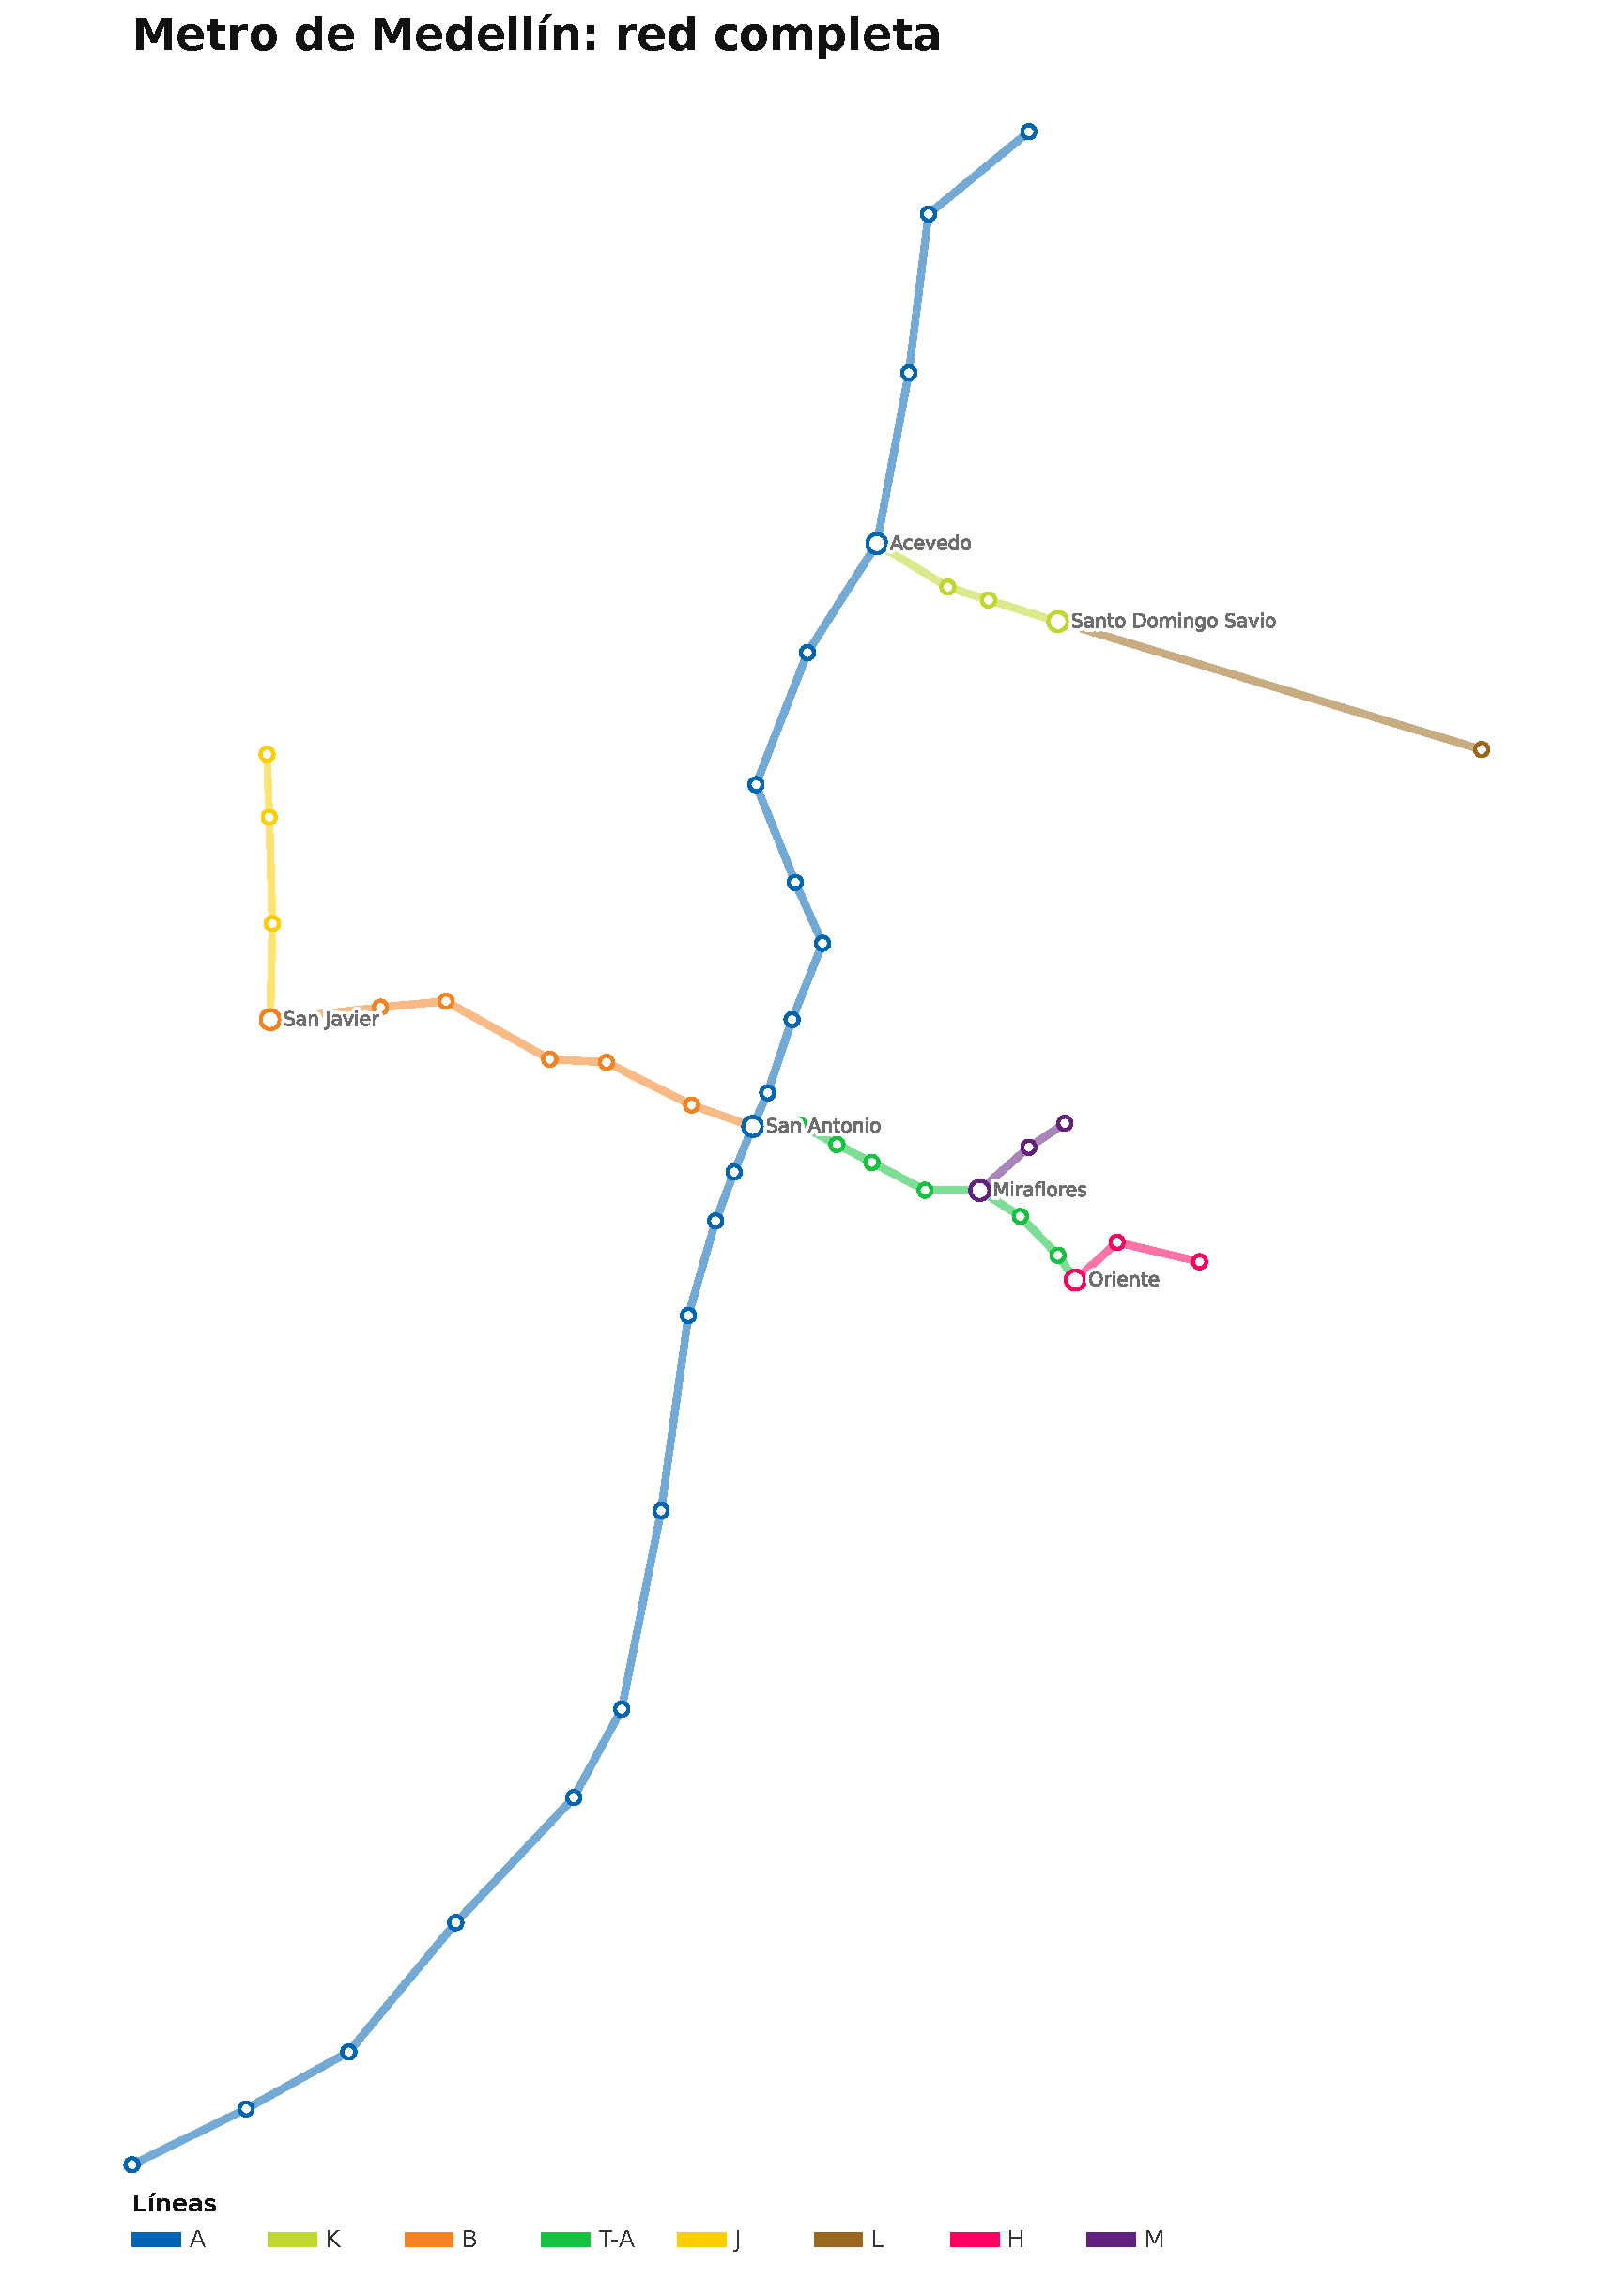
\includegraphics[width=0.78\textwidth]{fig_red.pdf}
\caption{La red completa: las ocho líneas con su color, los intercambiadores con círculo más grande y la convención de colores abajo. Los 46 puntos son las estaciones del CSV.}
\label{fig:red}
\end{figure}

\subsection{DOT y JSON}

El DOT es un \arch{digraph} con un nodo por par (estación, línea), etiquetado con
el nombre y el color de su línea. Una arista por par de nodos (se filtra con
\arch{u < destino} para no dibujar las dos direcciones), con el tiempo en minutos
como etiqueta; las de transbordo van punteadas y la ruta seleccionada, en negro y
más gruesa. Así el archivo se abre en Graphviz o en cualquier visor de DOT y la
ruta se distingue a simple vista.

El JSON guarda tres bloques: \arch{estaciones} (id, nombre, líneas, lat, lon),
\arch{lineas} (código y color) y \arch{aristas} a nivel de estación (origen,
destino, minutos, tipo y línea). Cuando hay una ruta seleccionada agrega
\arch{ruta} con el origen, el destino, el total en minutos, la lista de estaciones
y la lista de tramos con su línea. Si no hay ruta, el campo vale \arch{null}.


% ===========================================================================
\section{Interfaz web}

\paragraph{Por qué.}
El menú de consola sirve para probar cada función, pero para mirar la red y
comparar rutas un mapa es mejor. La interfaz web es una capa sobre el mismo
motor: no reimplementa ningún algoritmo, solo dibuja lo que el C++ calcula.

\paragraph{El servidor (405 líneas).}
\arch{src/servidor.cpp} levanta un servidor HTTP con sockets POSIX
(\arch{socket}, \arch{bind}, \arch{listen}, \arch{accept}) en un solo hilo, que
atiende una petición a la vez. Solo acepta \arch{GET} y responde con
\arch{Connection: close}, que es todo lo que necesita un navegador y una persona.
La API devuelve JSON armado con \arch{ostringstream}, igual que la exportación:

\begin{center}
\footnotesize
\begin{tabular}{@{}p{4.7cm}p{9.8cm}@{}}
\toprule
Ruta & Qué devuelve \\
\midrule
\arch{/api/grafo} & líneas con su color, las 46 estaciones y los 45 tramos \\
\arch{/api/estaciones?q=san} & coincidencias del Trie para el autocompletado \\
\arch{/api/ruta} & hasta $k$ rutas con sus paradas y tiempos acumulados, más la comparación A*/Dijkstra; recibe origen, destino, $k$, transbordo y estación cerrada como parámetros \\
\arch{/api/articulacion} & los puntos de articulación de la red \\
\bottomrule
\end{tabular}
\captionof{table}{Los cuatro puntos de la API. El grafo se serializa una sola vez al arrancar; solo se reconstruye si el usuario cambia la penalización de transbordo.}
\end{center}

\paragraph{El mapa (715 líneas).}
\arch{web/index.html} es un solo archivo con todo el CSS y el JavaScript en
línea: no hay CDN ni tipografías externas, así que la interfaz funciona sin
internet. El dibujo se construye en el navegador con la misma proyección del
SVG exportado (longitud corregida por el coseno de la latitud, latitud
invertida), y encima se agregan capas para las líneas, las estaciones, la ruta y
los rótulos. El mapa se puede arrastrar y acercar con la rueda o con los botones;
al hacer clic en una estación se fija el origen y con el segundo clic el destino
(figura~\ref{fig:web}).

\paragraph{Los controles.}
El panel izquierdo repite las opciones del menú: el deslizador de transbordo
(de 0 a 10 minutos) obliga al servidor a reconstruir el grafo y recalcula la
ruta en el momento, el selector de Yen pide hasta 6 rutas, el desplegable de
estación cerrada simula el cierre y una casilla marca los puntos de articulación
con un anillo punteado. Debajo del resultado aparece la comparación A* contra
Dijkstra: los nodos explorados por cada uno, en número y en barra, con el tiempo
en microsegundos.

\paragraph{Dónde queda el cálculo.}
El JavaScript no calcula rutas: solo pide JSON y pinta. La tentación era portar
Dijkstra a JavaScript para que la página funcionara sola, pero habría dejado dos
implementaciones del mismo algoritmo y la del informe ya no sería la que se usa.
El servidor resuelve eso con unas pocas líneas de sockets.

\begin{figure}[htbp]
\centering
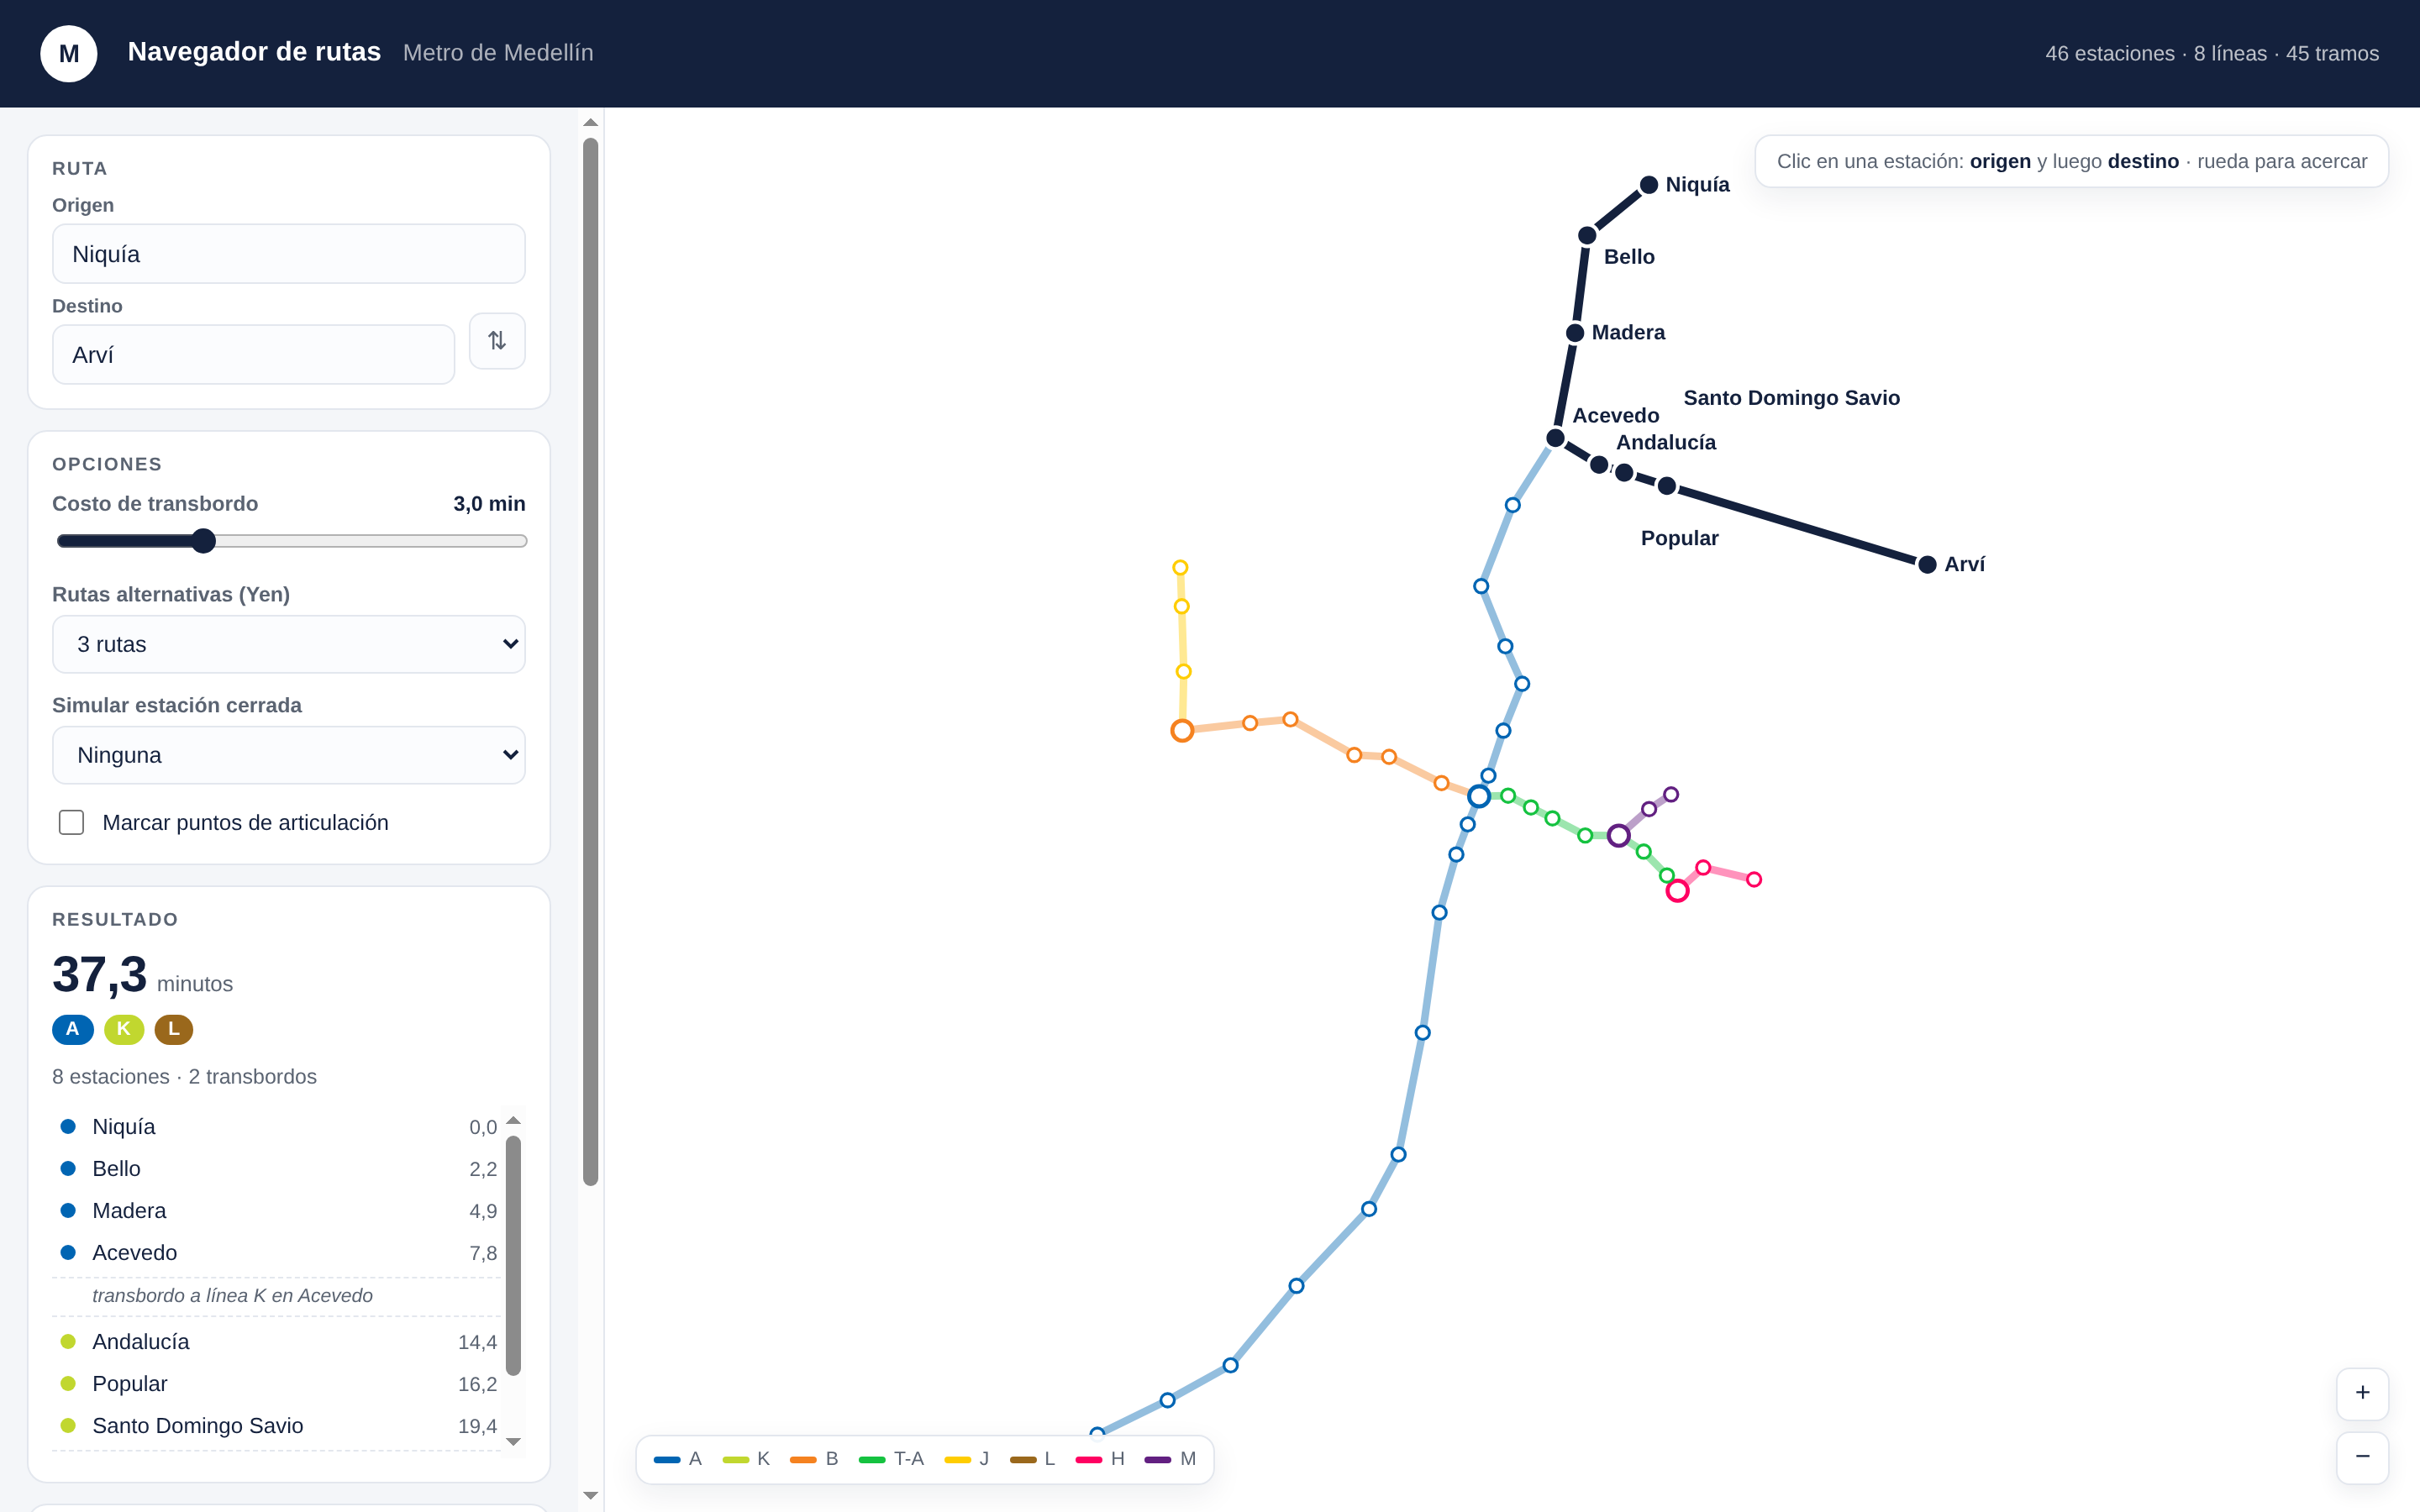
\includegraphics[width=\textwidth]{fig_web.png}
\caption{La interfaz web con la ruta Niquía → Arví (37,3 minutos, dos transbordos). A la izquierda el panel con el origen, el destino, el deslizador de transbordo, las rutas alternativas y la lista de paradas con su tiempo acumulado; a la derecha el mapa con la ruta en oscuro y los nombres de las estaciones de la ruta.}
\label{fig:web}
\end{figure}

% ===========================================================================
\section{Resultados}

\subsection{Rutas de ejemplo}

\begin{center}
\small
\begin{tabular}{lrrrl}
\toprule
Ruta & Tramos & Transbordos & Minutos & Líneas \\
\midrule
Niquía → Arví              &  7 & 2 & 37,3 & A, K, L \\
La Aurora → Miraflores     & 14 & 2 & 36,3 & J, B, T-A \\
San Javier → Santo Domingo & 16 & 2 & 35,5 & B, A, K \\
Niquía → La Estrella       & 20 & 0 & 40,2 & A \\
\bottomrule
\end{tabular}
\captionof{table}{Cuatro rutas calculadas por el programa. Los tramos no cuentan los transbordos.}
\label{tab:rutas}
\end{center}

Las dos primeras están en las figuras~\ref{fig:arvi} y \ref{fig:miraflores}. La
de La Aurora a Miraflores es la que más líneas usa de las cuatro (tres) y pasa
por 15 estaciones: baja por el cable J hasta San Javier, cruza en la B hasta San
Antonio y sigue en el tranvía.

\begin{figure}[htbp]
\centering
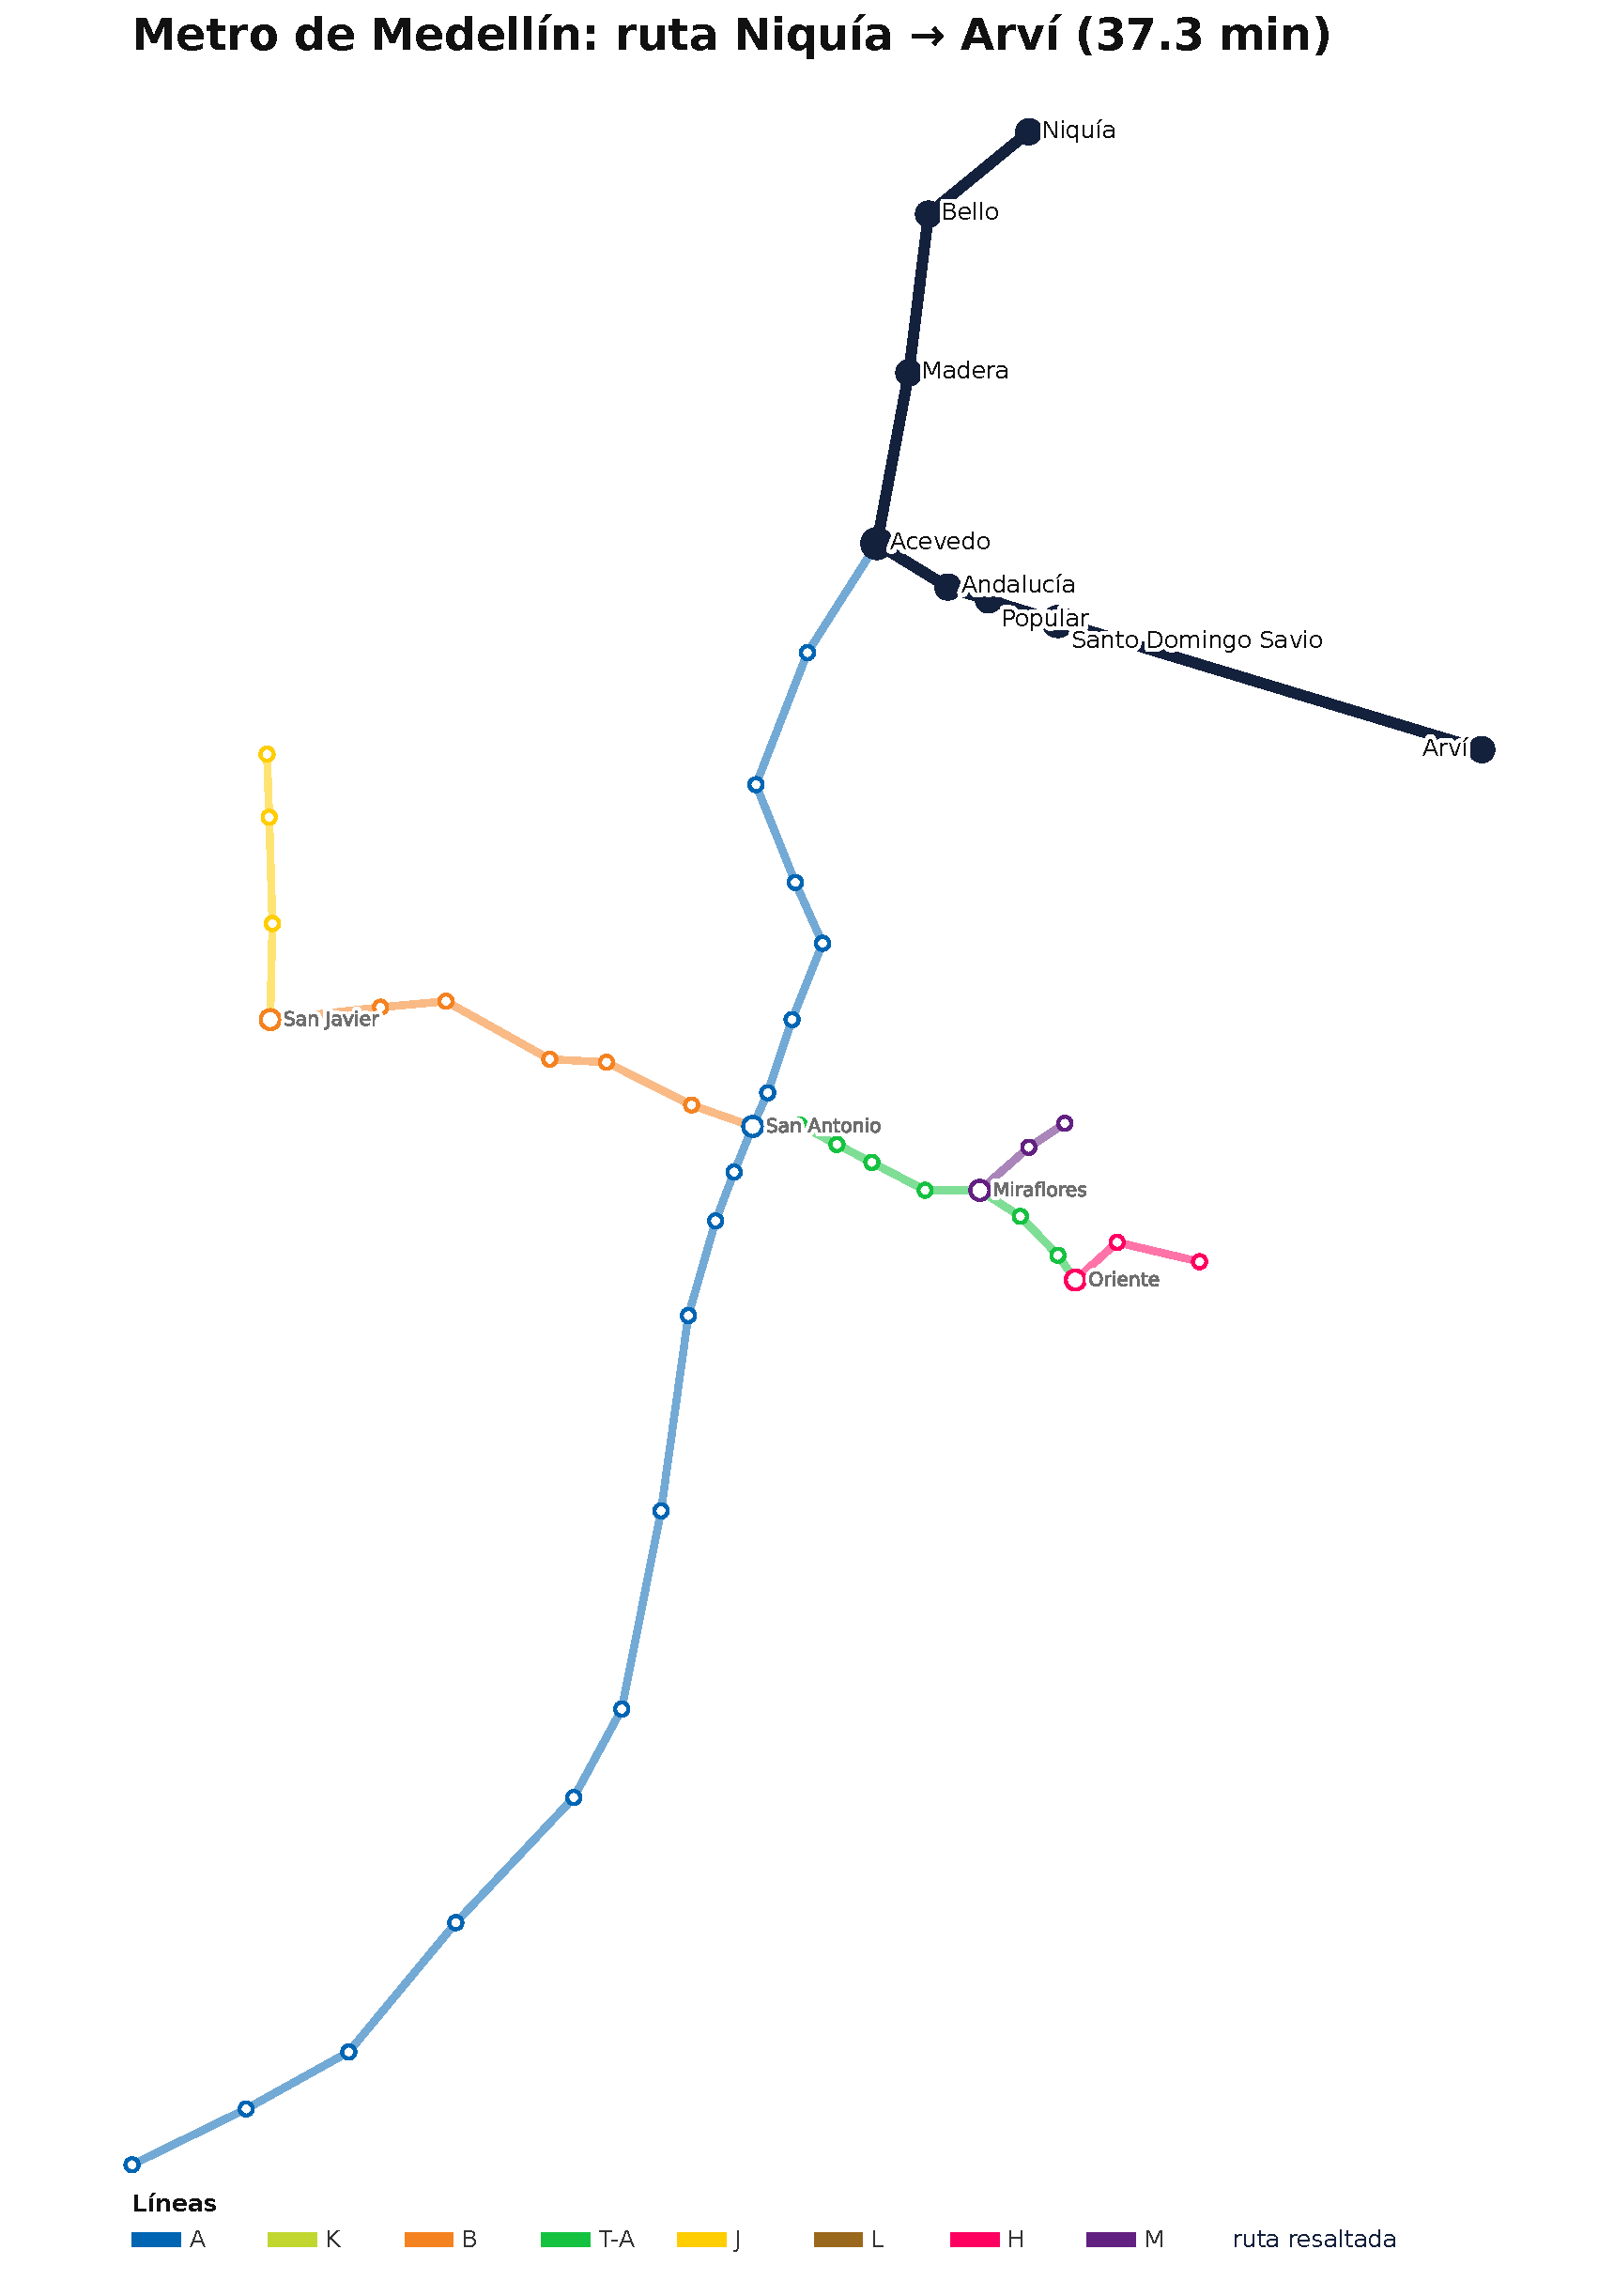
\includegraphics[width=0.86\textwidth]{fig_ruta_arvi.pdf}
\caption{Ruta Niquía → Arví: 37,3 minutos. En oscuro la ruta; se ven los dos transbordos, en Acevedo (A a K) y en Santo Domingo Savio (K a L), donde el cable L sale hacia el oriente.}
\label{fig:arvi}
\end{figure}

\begin{figure}[htbp]
\centering
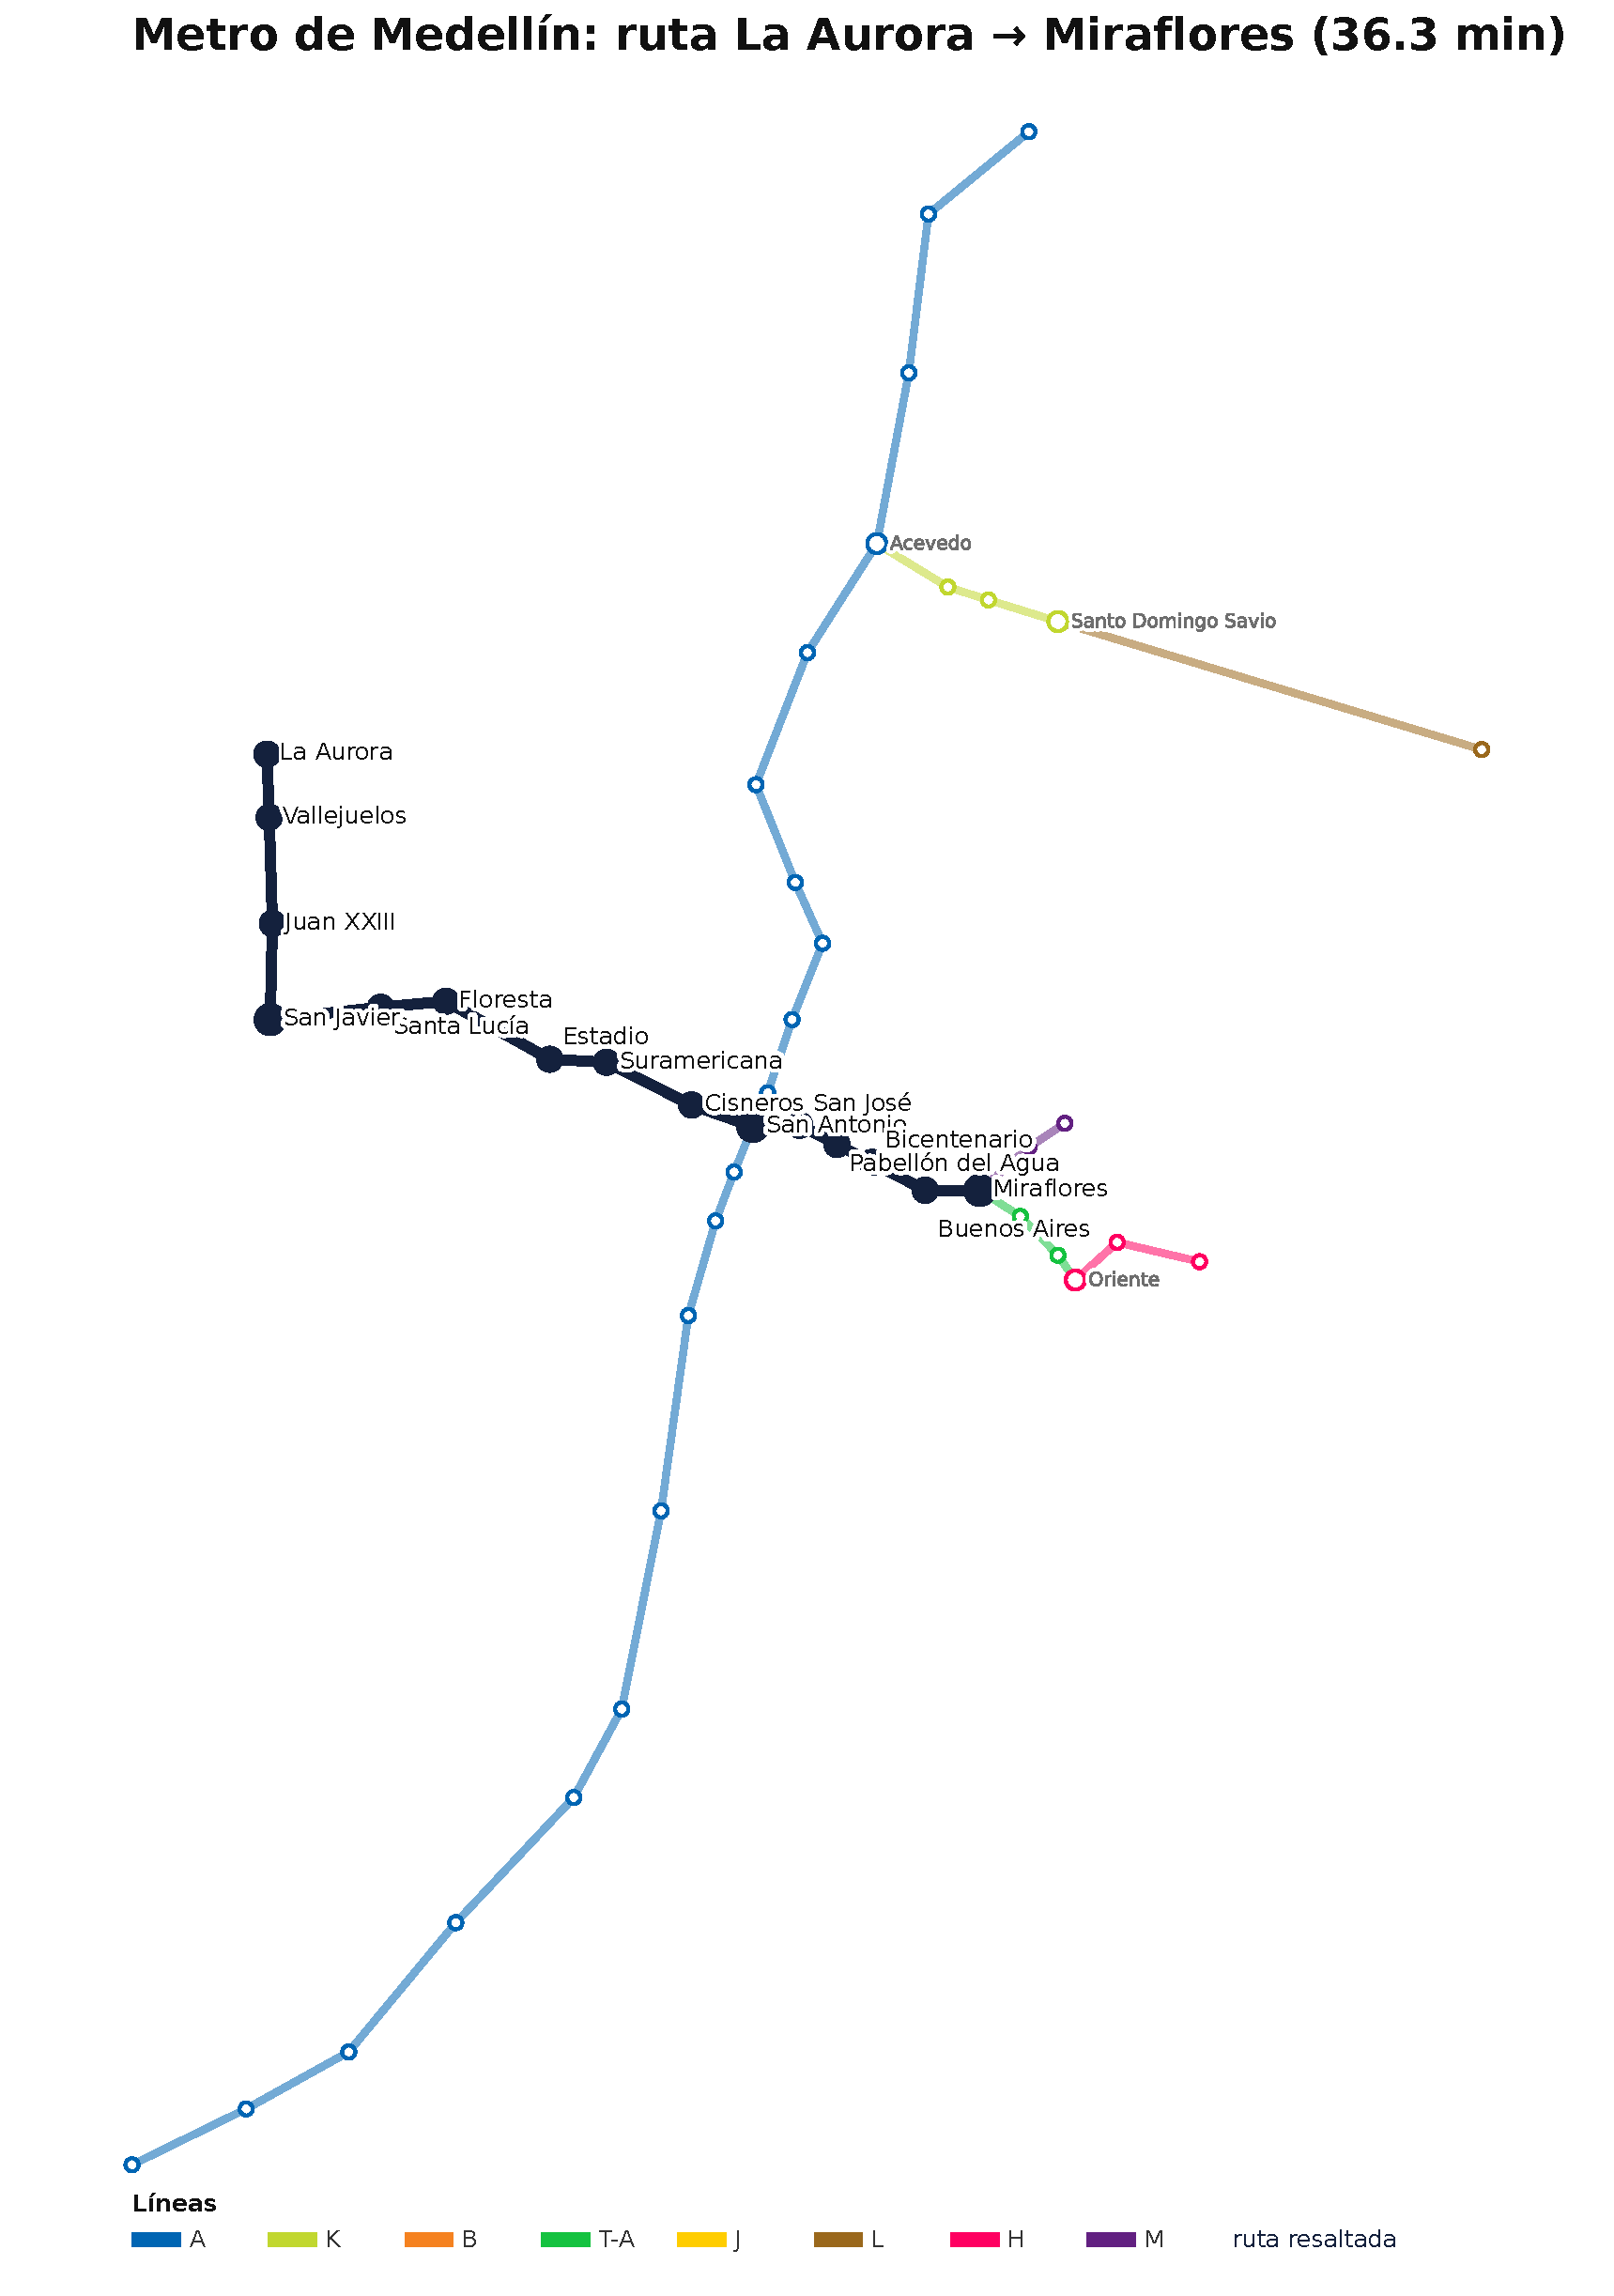
\includegraphics[width=0.86\textwidth]{fig_ruta_miraflores.pdf}
\caption{Ruta La Aurora → Miraflores: 36,3 minutos y tres líneas. El tramo recto del centro es la B entre San Javier y San Antonio; de ahí sale el tranvía hacia el oriente.}
\label{fig:miraflores}
\end{figure}

\subsection{Las pruebas}

\arch{tests/test\_main.cpp} usa solo \arch{assert}: no hay framework. Verifica la
estructura cargada (46 estaciones, 8 líneas, 53 nodos), las cuatro rutas sumadas a
mano, la simetría de los tiempos (La Estrella → Niquía cuesta lo mismo que al
revés), que A* y Dijkstra den el mismo costo en 20 pares, que Yen devuelva tres
rutas en un grafo con ciclo, que Acevedo y Santo Domingo Savio sean de articulación
y La Estrella no, que sin Santo Domingo no se llegue a Arví, que la penalización
de transbordo se aplique exacta y que el Trie ignore tildes y mayúsculas. Las
pruebas compilan con \arch{-UNDEBUG} para que \arch{NDEBUG} de \arch{Release} no
las desactive en silencio.

% ===========================================================================
\section{Limitaciones}
\label{sec:limitaciones}

\begin{enumerate}
  \item \textbf{Los tiempos son estimados.} Salen de la ecuación~\eqref{eq:tiempo}
        con una velocidad comercial por línea. No incluyen la espera del tren ni
        las frecuencias (2:50 min en hora pico en la A, más en hora valle), que en
        un viaje con transbordos puede pesar más que los minutos de viaje. Tampoco
        distinguen hora pico de hora valle.
  \item \textbf{La red es un árbol.} 46 estaciones y 45 tramos, sin ciclos. Por eso
        Yen devuelve una sola ruta entre cualquier par y 40 de las 46 estaciones
        son puntos de articulación. Las alternativas reales en Medellín vienen de
        los buses del SIT y de Metroplús, que no modelamos.
  \item \textbf{Las coordenadas son las publicadas, no medidas.} Cinco cifras
        decimales dan precisión de metros, suficiente para dibujar y para estimar
        distancias, pero un tramo real no es una recta entre dos estaciones: el
        SVG dibuja segmentos rectos y no la geometría de la vía.
  \item \textbf{El transbordo es un número.} Los 3 minutos no distinguen entre
        cambiar de andén en San Antonio y caminar hasta el tranvía, ni dependen de
        la estación. El modelo es el mismo para todos los intercambiadores.
  \item \textbf{A* no gana en tiempo a esta escala.} Explora menos nodos, pero el
        cálculo de la heurística cuesta más que lo que ahorra en un grafo de 53
        nodos. La comparación honesta es la de nodos explorados.
  \item \textbf{Yen no está validado sobre datos reales con ciclos}, porque no los
        hay. Queda validado sobre un grafo sintético en las pruebas; si se
        agregaran líneas que cerraran un ciclo, el algoritmo ya está listo.
  \item \textbf{El grafo es estático.} No hay horarios, ni cierres temporales por
        hora, ni estaciones con acceso restringido, ni costos por tipo de usuario.
\end{enumerate}

% ===========================================================================
\section{Conclusiones}

\begin{enumerate}
  \item Las cuatro funcionalidades mínimas están y se pueden ver correr: carga del
        grafo desde CSV, ruta de menor tiempo con Dijkstra, SVG con la ruta
        resaltada y exportación a DOT y JSON.
  \item Modelar los nodos como pares (estación, línea) es lo que permite que el
        transbordo sea una decisión del algoritmo y no una suma posterior. Cuesta
        53 nodos en vez de 46 y 16 aristas más, y a cambio el camino óptimo ya
        tiene en cuenta el cambio de línea.
  \item La heurística haversine dividida por la velocidad máxima es admisible por
        la desigualdad triangular, y se ve en los datos: A* y Dijkstra dan el mismo
        costo en los 20 pares y A* explora el 64,3\,\% de los nodos. En un grafo
        de este tamaño el ahorro no se traduce en tiempo de reloj.
  \item La forma de la red manda. Que sea un árbol explica a la vez el resultado de
        Yen (una sola ruta), el de los puntos de articulación (40 de 46) y el de la
        estación cerrada (Arví queda aislado si se cierra Santo Domingo Savio). Tres
        funcionalidades distintas dicen lo mismo sobre la topología.
  \item La interfaz web confirma que la separación sirve: el servidor expone el
        motor por HTTP y la página solo dibuja. Agregar el mapa interactivo no
        obligó a tocar Dijkstra, A*, Yen ni el Trie.
  \item Los datos son la parte más frágil del proyecto. Los nombres y las
        coordenadas se pueden verificar, pero los tiempos no son oficiales y la
        espera no está modelada. Cualquier conclusión sobre planes de viaje reales
        tiene que empezar por ahí.
\end{enumerate}

% ===========================================================================
\appendix

\section{Compilación y salidas reales}
\label{anexo:compila}

Compilación completa desde cero, sin advertencias:

\begin{lstlisting}[style=term]
$ cmake -S . -B build && cmake --build build -j4
-- Configuring done
-- Generating done
-- Build files have been written to: .../build
[ 87%] Built target nucleo
[100%] Built target pruebas
[100%] Linking CXX executable navegador
[100%] Built target navegador

(sin advertencias: grep -c warning sobre la salida completa del build da 0)
\end{lstlisting}

El mismo código se compiló también para Windows con MinGW-w64 (GCC 12),
indicándole a CMake que el sistema destino es Windows, y tampoco produjo
advertencias: genera \arch{navegador.exe} y \arch{pruebas.exe}. Ese paso es el
que ejercita de verdad el bloque \arch{\#ifdef \_WIN32} de
\arch{src/servidor.cpp} y el enlace contra \arch{ws2\_32}.

Las pruebas:

\begin{lstlisting}[style=term]
$ ./build/pruebas
OK estructura del grafo
OK rutas conocidas
OK simetría
OK A* = Dijkstra en 20 pares
OK rutas alternativas (1 en la red, 3 en el grafo con ciclo)
OK puntos de articulación (40)
OK estación cerrada
OK penalización de transbordo
OK autocompletado con Trie
Todas las pruebas pasaron
\end{lstlisting}

Una consulta completa, con la salida tal como la imprime el programa:

\begin{lstlisting}[style=term]
$ ./build/navegador
Metro de Medellín: 46 estaciones, 8 líneas, 53 nodos (estación, línea), 106 aristas dirigidas

Ruta Niquía -> Arví
  Niquía
  Bello  [Línea A]  2.2 min
  Madera  [Línea A]  4.9 min
  Acevedo  [Línea A]  7.8 min
  -- transbordo a Línea K (+3.0 min) en Acevedo
  Andalucía  [Línea K]  14.4 min
  Popular  [Línea K]  16.2 min
  Santo Domingo Savio  [Línea K]  19.4 min
  -- transbordo a Línea L (+3.0 min) en Santo Domingo Savio
  Arví  [Línea L]  37.3 min
Total: 37.3 min | 7 tramos | 2 transbordos | 8 estaciones
Nodos explorados: 44 | tiempo de búsqueda: 0.003 ms
\end{lstlisting}

\section{Mapa de archivos}
\label{anexo:mapa}

\begin{center}
\footnotesize
\begin{tabular}{lrp{8.4cm}}
\toprule
Archivo & Líneas & Contenido \\
\midrule
\arch{graph.hpp}      &  80 & estructuras (Estacion, Linea, Nodo, Arista, Tramo) y la clase Graph \\
\arch{graph.cpp}      & 151 & normalización de texto, haversine, consultas del grafo, tramos de una ruta \\
\arch{algorithms.hpp} &  43 & Resultado, Bloqueo y las firmas de los algoritmos \\
\arch{algorithms.cpp} & 330 & Dijkstra (53), A* (115), Yen (197), puntos de articulación (276) \\
\arch{trie.hpp}       &  79 & Trie con los métodos en línea \\
\arch{io.hpp}         &  16 & carga y exportación \\
\arch{io.cpp}         & 485 & CSV (87), DOT (177), JSON (232), SVG (317) \\
\arch{servidor.hpp}   &   8 & firma de \arch{iniciarServidor} \\
\arch{servidor.cpp}   & 405 & servidor HTTP con sockets y API JSON \\
\arch{web/index.html} & 715 & interfaz web: mapa interactivo, panel de controles y comparación \\
\arch{main.cpp}       & 447 & menú de consola y modo \arch{--web} \\
\arch{tests/test\_main.cpp} & 153 & nueve bloques de \arch{assert} \\
\arch{CMakeLists.txt} &  37 & biblioteca \arch{nucleo}, \arch{navegador}, \arch{pruebas} y los flags \\
\arch{data/stations.csv} & 47 & 46 estaciones con id, nombre, líneas, lat y lon \\
\arch{data/edges.csv}    & 46 & 45 tramos con origen, destino y minutos \\
\bottomrule
\end{tabular}
\captionof{table}{Archivos del proyecto. Los números de línea de la tercera columna son los que usan los listados de este informe.}
\end{center}

\noindent
Los listados de las secciones anteriores se insertan con \arch{\textbackslash
lstinputlisting} directamente desde los archivos, con rangos de línea, así que el
código del informe es el que se compiló y se ejecutó.

\end{document}
